%%
%% This is file `Author_Handbook_Body.tex'
%% 
%% Copyright 2017 American Mathematical Society.
%% 
%% This file is part of the collection comprising the AMS Author Handbooks.
%% For details and license information, see the file README-AH.txt.
%%
%% The Current Maintainer of this work is the American Mathematical
%% Society.
%% 
%% ========================================================================
%% 
%% This is the body of the Handbook; it will be called from
%% a separate driver from each of the four document categories.

%% Bypass the amsbook \maketitle formatting to obtain a
%% more informative title page, derived from the style
%% used for the previous handbook.

\begin{document}

\frenchspacing

%\maketitle

\thispagestyle{empty}
\vspace*{1.25in}
\noindent
\begin{minipage}[t][5.5in]{\textwidth}
 \centering
 {\Huge\bfseries AMS Author Handbook\\[4pt]
  \jmpm{Journal Classes}{Monograph Classes}
  {Proceedings and Collections Classes}{Memoirs Class}\par}
 \vspace{.5in}
 {\LARGE September 2017}\par
 \vspace{\fill}
 American Mathematical Society\\
 201 Charles Street\\
 Providence, RI \ 02904-2294 \ USA\\[1\baselineskip]
 \href{http://www.ams.org/authors}{\texttt{www.ams.org/authors}}
\end{minipage}

%\cleardoublepage
\clearpage

%% Arrange the two TOC pages side by side when bound.
\makeatletter
\@openrightfalse
\makeatother

\tableofcontents

%% Avoid a blank right-hand page before the one-page introduction,
%% except for monographs, which has a two-page introduction, or if
%% openany has been specified as the documentclass option.
\ifmonograph
 \makeatletter
 \if@openany
 \else \@openrighttrue
 \fi
 \makeatother
\fi

\chapter{Introduction}

This handbook is directed mainly to authors preparing material for
publication by the \AMS\ (AMS), using \amslatex/ document classes.
As such, it deals with the AMS publishing style.  Since these document
classes are also used by authors who are not submitting items to the AMS,
the handbook also covers topics of more general relevance.  However, it
assumes familiarity with standard \latex/ techniques and conventions,
and contains only material specific to AMS packages.

The tagging of elements in a manuscript---title, author(s), section
headings, theorems, etc.---is consistent through all AMS author packages,
and the structure of elements in the body is based on that of the original
\latex/ document classes.
Thus a manuscript prepared using an appropriate generic document class
can be modified trivially to use a more specific AMS document class simply
by updating the \cn{documentclass} statement and making a few adjustments
to the tagging of data in the top matter.
\ifmemoirs
 For the \textit{Memoirs of the American Mathematical Society}, use
 \Verb+\documentclass{memo-l}+.
\else
 For example, specify 
 \ifjournal {the journal \textit{Proceedings of the American Mathematical
  Society} as follows: {\Verb+\documentclass{proc-l}+}}. \fi
 \ifmonograph {the \textit{Graduate Studies in Mathematics} monograph series
  as follows: \Verb+\documentclass{gsm-l}+}. \fi
 \ifproceedings {the \textit{Proceedings of Symposia in Pure Mathematics}
  proceedings series as follows: \Verb+\documentclass{pspum-l}+}. \fi
\fi
(The \Verb+-l+ in the \cn{documentclass} name is an ``ell'', for \latex/,
not a ``one''.)

\jmp{\input J-Series}{\input M-Series}{\input PC-Series}

\ifmemoirs
  The \amslatex/ package is available from:
\else
  The \amslatex/ packages are available from:
\fi

\begin{center}
\jmpm
{\href{http://www.ams.org/authors/journalpackages}{\texttt{www.ams.org/authors/journalpackages}}}%
{\href{http://www.ams.org/authors/monopackages}{\texttt{www.ams.org/authors/monopackages}}}%
{\href{http://www.ams.org/authors/procpackages}{\texttt{www.ams.org/authors/procpackages}}}%
{\href{http://www.ams.org/authors/journalpackages}{\texttt{www.ams.org/authors/journalpackages}}}
\end{center}

\noindent For more information, see Chapter~\ref{ch:resandhelp}.

\ifproceedings
 \bigskip

 \textbf{Note to editors of proceedings volumes:}\\
 Instructions for preparing the front matter are presented in the 
 \href{http://http://www.ams.org/publications/books/collproc/editpkg}%
 {AMS Editor's Package} (\url{www.ams.org/publications/editpkg})

\newpage
\fi

\ifjournal \newpage \fi

%%%%%%%%%%%%%%%%%%%%%%%%%%%%%%%%%%%%%%%%%%%%%%%%%%%%%%%%%%%%%%%%%%%%%%%%

\ifmonograph

\clearpage

\section*{The basics}

%\noindent
A monograph is a long work by a single author or co-authors on a
single subject.  Each chapter should be prepared as a separate file,
as should the bibliography.  In addition, a ``driver'' file should be
used to input all the others.  These files should be given meaningful
names, so that when they are transmitted to the AMS, there will be no
question about which file represents which chapter.  For example, a
monograph by author Grey might be composed of files named
\filnam{grey.tex} (the driver file), \filnam{grey-ch1.tex},
\filnam{grey-ch2.tex}, \dots, \filnam{grey-ch12.tex},
\filnam{grey-appa.tex}, etc., and \filnam{grey-bib.tex} (or
\filnam{grey.bbl} if \bibtex/ is used).
If the author name is a common one, please include something to make
it unique, such as first initials.

Information that identifies the author(s), the subject matter of the
monograph, acknowledgments of support, and so forth, will appear in the
front matter of the book.  Place this information in the driver file,
%and use the tags shown below.  Most of these are the same as the tags
and use the tags shown in Table~\ref{tbl:1} in the
\textit{\nameref{s:topmatter}} section (page~\pageref{s:topmatter}).
This section provides
explanations and an indication of which tags are required.
Most of the tags used for the top matter of a monograph are the same
as the tags associated with the top matter of an article.

This information will be provided to online bibliographic services
for indexing.

\fi % end \ifmonograph

\makeatletter
\if@openany
\else \@openrighttrue
\fi
\makeatother

%%%%%%%%%%%%%%%%%%%%%%%%%%%%%%%%%%%%%%%%%%%%%%%%%%%%%%%%%%%%%%%%%%%%%%%%

\section*{What's in it for the author?}

If the guidelines in this handbook are followed, there are some
clear benefits.
\begin{itemize}
\item The time between receipt of the manuscript and publication
  will be minimized.
\item The opportunity for introducing unintended errors will be
  greatly reduced.
\end{itemize}

As author, \emph{you} are responsible for the content of your
\jmpm{paper}{book}{paper}{\Memo}.  At the production end, the concern
is to turn the (electronic) manuscript into a published document in
the style of the
\ifmemoirs \Memos;
\else
 designated \jmp{journal}{book series}{book series};
\fi
this
\ifmemoirs
\else increasingly
\fi
includes various electronic outputs that
\bookseries{may }%
involve (automatic) conversion to non-\latex/ forms.  Use of standard
packages and elimination of unneeded material from your files (unused
macro definitions and packages, and commented text) will reduce the
need for technical tinkering.

If you have special requirements, assistance can be requested---%
\emph{before} submission of your files---from the technical support
group; their email address is given on page~\pageref{ch:resandhelp}.


%%%%%%%%%%%%%%%%%%%%%%%%%%%%%%%%%%%%%%%%%%%%%%%%%%%%%%%%%%%%%%%%%%%%%

\chapter{Using the
 \protect\jmpm{AMS journal classes}{AMS monograph classes}%
 {AMS proceedings and collections classes}{AMS \Memos\ class}}

\ifmemoirs
\markleft{USING THE AMS \MEMOS\ CLASS}
\fi

\section{The basic checklist}\label{sec:check}
\noindent Some basic principles are important for effective handling of
 electronic submissions. Keep these principles in mind when preparing and
 submitting your files.

\begin{itemize}

\item Use the \textbf{template} supplied in the author package for
 \ifmemoirs
  the \Memos; this will call the \verb+memo-l+ document class.
 \else
  your particular publication and the appropriate document class.
 \fi

\item Copy this template to a file with a name suitable to identify
 your document.  File names should not exceed 20 characters in length,
 and consist only of numeric or unaccented alphabetic (ASCII) characters.
 Avoid overly generic file names such as
 \jmpm{\texttt{article.tex}}{\texttt{chap1.tex}}%
 {\texttt{article.tex}}{\texttt{chap1.tex}},
 \texttt{mybib.tex} or \texttt{fig1.eps}.

\item Do not modify page sizes or other \textbf{dimensions}.
 Page sizes must conform to the specifications of the
 \ifmemoirs \Memos.
 \else
  publication for which you are preparing your manuscript.
 \fi
 The text width is determined by the trim size of the publication, and
 use of a larger text width for the file you submit guarantees that
 line breaks will change in the final printed version.  This is
 especially critical for math displays, and also affects tables and
 figures.

\item Do not modify the default \textbf{font size}, except temporarily
 for proofreading your work.  As with text width, any change will result
 in different line breaks in the final version.

\item Use only \textbf{``public'' packages} available from
 \href{http://www.ctan.org/search.html}{CTAN} (the Comprehensive
 \TeX\ Archive Network).

\item All of the AMS document classes incorporate the code for the AMS
 theorem (\pkg{amsthm}) package and automatically load the \pkg{amsmath}
 package.  It is not necessary to request either one explicitly.
 Except for a brief overview of how to activate theorems (see
 page~\pageref{ss:thmsetup}), the details will not be repeated here;
 see the user guides for these packages \cite{ATH,AMG}.
 The \pkg{amsfonts} package is loaded
 as well, unless the \opt{noamsfonts} option is specified; see the
 AMSFonts User's Guide \cite{AFG} for the features provided.

\item Do not redefine \textbf{any} existing \latex/ or \amslatex/
 commands.  Use \cn{newcommand}, not \cn{def}, to be warned if the
 name you have chosen is already in use.

\item Put \textbf{definitions} for frequently occurring mathematical
 expressions together \textbf{in the preamble}, before the start of the
 text of the manuscript.  Once a macro is created for an expression,
 use it for every occurrence of that expression, except as noted below.

\item Do not use \textbf{author-defined macros} in author names, titles,
 \notmonograph{abstract, }%
 section and theorem headings, or references; use only standard commands.
 Do not hard-code font changes.  Use \tex/ coding for special fonts
 (e.g., boldface or italic) only within the text of the manuscript.

\item Avoid the use of math in the title and in
\ifmonograph
 chapter and section
\else
 other
\fi
 headings.
 \textbf{Titles} are provided to on-line bibliographic services for indexing.
 Use of \tex/ math coding (especially dollar signs) will result in
 inaccurate bibliographic listings, and problematic PDF bookmarks.

\item Determine the \textbf{2010 Mathematics Subject Classification} numbers
 representing the primary and secondary subjects of the work.  A list of
 these numbers can be found on the web at
 \href{http://www.ams.org/msc}{\texttt{www.ams.org/msc}}.  Enter the
 information with \cn{subjclass[2010]} where indicated in the template.

\item Make sure that \textbf{graphics} do not extend into the margins%
 \ifmemoirs .
 \else ;
  the width of the text may vary depending on the
  \jmp{journal}{book series}{book series}.
 \fi
 Check that all graphics conform to the AMS graphics guidelines---see
 Chapter~\ref{ch:graphics}, page~\pageref{ch:graphics}.
 
\item Do not use \tex/ coding to control \textbf{line and page breaks}. Lines
 and pages may break differently in the published
 \jmpm{article}{book}{article}{\Memo} from the way
 they break in the file you submit.  If you insert \tex/ coding for
 line and page breaks, it will have to be removed for production.
 This work could offset any time saved by your keyboarding the
 manuscript, and any change to your \tex/ file creates a small chance
 of additional errors being introduced.

\item Avoid explicit horizontal and vertical \textbf{spacing commands}
 for the same reason.

\item For \textbf{displayed equations}, the AMS style requires equation numbers
 to be on the left, flush with the left margin. See
 section~\ref{ssec:eqnum}, page~\pageref{ssec:eqnum}.

\item Use \ttcs{cite} to indicate \textbf{citations} in the manuscript.
 \notmonograph{The \ttcs{cite} command may not appear in an abstract.}

\item Include all available information for \textbf{references}; use the
 abbreviations for journals and book series from \cite{ABMR}, either in
 print or on the web.
\ifmonograph
\else
 All references will be replaced in production by corresponding entries
 in \pkg{amsrefs} form drawn from \MSN\ (see section~\ref{sec:bibref},
 page~\pageref{sec:bibref}).
\fi

\item Include the research \textbf{address} or institutional affiliation
 and current address (if different) of each author.  Email addresses
 and URLs may be included optionally.  Email addresses will appear in
 \jmpm{articles}{books}{articles}{\Memos}
 posted online; URLs will not; both will appear in print.

\item \textbf{Proofread} your \jmpm{article}{book}{article}{\Memo}
 thoroughly and carefully.
\ifjournal
\else
 Publications in
 \ifmemoirs
  \Memos{}
 \else
  some book series
 \fi
 will not be given an editorial proofreading.
\fi

\item \textbf{Verify} that author-submitted source files exactly match
 the accepted reference copy of the
 \jmpm{article}{book}{article}{\Memo}.

\end{itemize}

%%%%%%%%%%%%%%%%%%%%%%%%%%%%%%%%%%%%%%%%%%%%%%%%%%%%%%%%%%%%%%%%%%%%%%%%

%  token expansions for use in individual checklists
%  used for journals and proceedings checklists

\FirstPageFootnotes{Unmarked, unnumbered \textbf{footnotes on the first page}
 of an article should include primary classification numbers according to
 the 2010 Mathematics Subject Classification scheme
 (\href{http://www.ams.org/msc}{\texttt{www.ams.org/msc}})
 (required); grant information (optional); and key words and phrases
 describing the subject matter of the article (optional). Formatting is
 automatic when using the AMS style files.
}

\ArticleTitleDesc{The first page of an article must contain a
 \textbf{descriptive title}.  This title should be short, but informative;
 avoid useless or  vague phrases such as ``some remarks about'' or
 ``concerning''.
}

\ArticleTitleUC{For \textbf{article titles}, only the first word, the
 first word after a `:' and proper nouns should be capitalized.
 Supply a shortened form of the title if the full title is too long
 for the running head, leaving space for the page number;
% which cannot exceed 24 picas (10 cm.).
 check the length by looking at the output.
}

\RunHeadJP{The \textbf{running heads} on the left-hand (even-numbered)
 pages will be generated from the author name(s) entered in the top
 matter.  Shortened forms must be provided if necessary to fit on one
 line, leaving room for the page number.  The resulting running heads
 should match the names as given on the first page.  Uppercasing will
 be applied automatically if you are using AMS style files.
}

\BiblioInFile{All \textbf{bibliographic data} must be incorporated into the
 article file.
 If you are using \pkg{amsrefs}, include this data in the appropriate place.
 If you are using \bibtex/, insert the contents of the \filnam{.bbl} file into
 your \filnam{.tex} file; do not send the \filnam{.bib} file.  Be aware that
 \bibtex/ data will be updated, in \pkg{amsrefs} form, by data drawn from
 \MSN.  These are called ``enhanced references'';
 see section~\ref{sec:bibref}, page~\pageref{sec:bibref}.
}

\AcadAffil{Academic or other \textbf{affiliations} should appear at the end
 of your article, after the bibliography or references.
 A \textbf{current address}, if different from the affiliation, should
 follow the affiliation on a separate line.
 An \textbf{email address} should be included if available.
 Addresses are part of the top matter in AMS author packages;
 formatting is taken care of automatically by the AMS style files.
}

%  used in monographs and Memoirs checklists

\UseDriverFile{Use a \textbf{driver file} and put the source code
 for each chapter in a separate file, using \ttcs{include}
 (not \ttcs{input}) to pull them together into a single document.
}

\ChapterRight{Ordinarily, every chapter must begin on a new right-hand
 (odd-numbered) page.
}

\ChapterTitleUC{In \textbf{chapter titles}, the
 first and last words of the title and all nouns, pronouns, adjectives,
 adverbs, and verbs should be capitalized; articles, conjunctions, and
 prepositions should be lowercased except for the first and last words
 of the title.
}

\RunHeadMM{The \textbf{running heads} on the left-hand (even-numbered)
 pages should have the chapter title%
 \monoormemo{; the exact style will be taken care of by the class file}%
 { in uppercase letters}.
 The title in running heads should be shortened only if necessary to fit
 on one line, leaving room for the page number.  The running heads on the
 right-hand (odd-numbered) pages should have the section title
 (shortened if necessary)%
 \monoormemo{ in the same style as the heading on left-hand pages}%
 { in uppercase letters}.  Uppercasing%
 \monoormemo{ or other styling}{} will be
 applied automatically if you are using AMS style files.
}

\BiblioBooks{All \textbf{bibliographic data}, if it is not already prepared
 using \pkg{amsrefs}, will be converted to \pkg{amsrefs} form, drawing data
 from \MSN\ when that exists.  This is to provide the data in consistent
 form to on-line bibliographic services, who may use it for indexing
 or to compile citation lists.
}

\AddHyperref{An AMS-specific version of the \pkg{hyperref} package will be
 added by AMS staff at the appropriate stage of the production process
 primarily for the purpose of adding PDF bookmarks.  This will also affect
 internal cross-references and external URLs.
}

\GrantsThanks{Give information on \textbf{grants} or contracts under which the
 research was performed, including grant number, using the \ttcs{thanks}
 command.
}

\ConsentToPublish={A \textbf{Consent to Publish and Copyright Agreement}
 is sent to the author(s)
%% although CTPs *are* sent out electronically, vwa wants to leave this open
% electronically
 when the accepted work is received at the AMS\@.
 Production of your work begins once the signed form is received by the
 AMS so attend to this as quickly as possible.  Authors retain the right
 to use all or part of their own work in future publications of their
 own.  They are, however, asked, but not required, to sign other rights over
 to the AMS\@.  If the author(s) transfers copyright to the AMS, the author(s)
 may dedicate their work to the public domain after 28 years from the date
 of publication; works in the public domain are not protected by copyright
 and can be used freely by everyone.
}

\jmpm{\input J-Checklist}{\input M-Checklist}{\input PC-Checklist}{\input Mem-Checklist}

%%%%%%%%%%%%%%%%%%%%%%%%%%%%%%%%%%%%%%%%%%%%%%%%%%%%%%%%%%%%%%%%%%%%%%%%

\section{The preamble}

The area between the \ttcs{documentclass} statement and the line
\verb+\begin{document}+ is referred to as the ``preamble''.  This is
the place to load external packages and define document-specific
commands.

\subsection{Document class options}

There are several \ttcs{documentclass} options authors might find useful.
Some restrictions that
\ifmemoirs
 are not relevant to the \Memos
\else
 may apply to particular 
 \jmp{journals}{book series}{book series}
\fi
are not presented here in detail%
\ifmemoirs .
\else
 , but can be found in the author package instructions for those
 publications.
\fi

%%  the following options are not described here:
%%   [e-only]
%%   [titlepage], [notitlepage]
%%   [onecolumn], [twocolumn]
%%   [nomath], [noamsfonts]. [psamsfonts]

\begin{itemize}

\item \textbf{Paper size} defaults to \opt{letterpaper}, and this
 is the size expected when files are submitted for publication.
 However, authors outside the U.S. may find \opt{a4paper} useful
 for preparing drafts.

\item \textbf{Two-sided or one-sided printing} defaults to
\opt{twoside}.  \opt{oneside} might also be useful for drafts,
 but should be removed when files are submitted for publication.

\item \textbf{Version} can be specified as \opt{draft} or \opt{final}.
 The \opt{draft} option causes overfull lines to be marked with a black
 slug  in the right margin, calling attention to problems that should be
 corrected before submission. The default option is \opt{final}.


\item The \textbf{font size} should not be changed from the default
\ifmonograph
 except by agreement with the Acquisitions Editor.  The usual default
 size is \opt{10pt}, but some series have a different default which is
 identified in the documentation for specific author packages.
\else \unskip, which is \opt{10pt}.
\fi
 If a larger size is desired for proofreading, options \opt{11pt} or
 \opt{12pt} are also available.  However, using a different size will
 affect line breaks, which is especially critical for displays or when
 math appears in text.  If a different size is used, reprocess your
 document before submitting files, and check and fix any bad breaks.

\ifmonograph
\item \textbf{Start on right- or left-hand page.}
 For most book series, chapters start on a right-hand page,
 but occasionally (when chapters are very short), starting on a
 left-hand page may be desirable.  The options \opt{openright} (default)
 and \opt{openany} control this arrangement.
\fi

\item \textbf{Equation numbering} defaults to the left, equivalent to
 \opt{leqno}.
 Numbering on the right, with \opt{reqno}, is also supported, but is
 strongly discouraged because it is incompatible with the marking of
 theorem endings with a \ttcs{qed} box at the right margin.

 For multiline equations, the equation number is by default centered
 vertically on the total height of the display (option \opt{centertags}).
 To make the equation number print on the first line (for left-hand
 numbers) or the last  line (for right-hand numbers), there is the
 option \opt{tbtags} (top/bottom).

\item \textbf{Flush left displays} can be specified by \opt{fleqn}.
 With this option, displayed equations are aligned on the left
 instead of centered, with an indentation of \ttcs{mathindent} from
 the left margin.

\end{itemize}

\subsection{Packages}
%%
The AMS document classes incorporate the code for the AMS theorem
(\pkg{amsthm}) package and automatically load the \pkg{amsmath}
package.  It is not necessary to request either one explicitly.
The user guides for these packages \cite{ATH,AMG} contain the details,
which will not be repeated here, but see section~\ref{ss:thmsetup}
for suggestions on setting up theorems.  The \pkg{amsfonts} package
is loaded as well, unless the \opt{noamsfonts} option is specified;
see the AMSFonts User's Guide \cite{AFG} for the features provided.

Not all publicly available packages are compatible with the AMS
document classes.  For this reason, we mention some that are:
\begin{itemize}
\item \pkg{amssymb} provides names for additional symbols from the
 AMS symbol fonts; see \cite{AFG} for details.
\monomemo{\item \pkg{amsbooka} provides the ability to specify a different
 or additional author for an individual chapter or appendix, and have that
 information automatically included in the TOC in an appropriate format.}
\monomemo{\item \pkg{amsmidx} supports multiple indexes for a book;
 an alternative package, \pkg{imakeidx}, may also be used, with
 some restrictions; see page~\pageref{ss:indexing}.}
\monomemo{\item \pkg{chngcntr} provides the command \cn{counterwithout}
 that can be used to undo a default counter resetting.  For example,
 \cn{counterwithout\{footnote\}\{chapter\}} will cause footnotes to be
 numbered continuously through a book, not reset for every chapter.}
\item \pkg{graphicx} is part of the \latex/ suite, preferred for
 inclusion of graphics.
\item \pkg{longtable} facilitates tables longer than one page.
\item \pkg{mathrsfs} (Ralph Snith's formal script, \cn{mathscr}) defines
 a script font that some authors prefer to the default \cn{mathcal}.
\item \pkg{mathtools} provides some display math enhancements that
 weren't anticipated when \pkg{amsmath} was developed.
\item \pkg{natbib} supports author-year referencing, appropriate for
 historical and expository works, when used with \bibtex/.
 \pkg{amsrefs} has a comparable facility.
\item \pkg{upref} forces cross-references with \cn{ref} to roman (upright);
 see ``Roman type'', page~\pageref{ss:roman}.
\item \pkg{tikz} is recommended for creating charts and other graphics,
 including commutative diagrams.
\item \pkg{xypic} is also recommended for creating commutative diagrams.
\end{itemize}
Some of these recommendations are noted in the templates that are
included in every author package.

There are several packages that cause particular problems for AMS
production.  Their use should be avoided:
\begin{itemize}
\item \pkg{biblatex} is not supported by the AMS production stream, and
  requires that a bibliography be converted to a compatible form, opening
  a path for potential errors.
\item \pkg{epsfig} has been superseded by \pkg{graphicx}.
\item \pkg{diagrams}, by Paul Taylor, contains a ``time bomb'' that
  renders it inappropriate for a production environment.
\item \pkg{geometry} changes page dimensions even if no explicit
  changes are specified by the author.
\item \pkg{microtype} is not supported by the AMS production stream,
  which relies on dvi output for automated graphics checking.
\item \pkg{makeidx} facilities are already in AMS document classes.
\item \pkg{parskip} redefines the processing of tables of contents, as
  well as making other format changes that do not follow AMS guidelines.
\end{itemize}

Don't load any packages that aren't actually needed.

%%%%%%%%%%%%%%%%%%%%%%%%%%%%%%%%%%%%%%%%%%%%%%%%%%%%%%%%%%%%%%%%%%%%%%%%

\subsection{New commands}
%%
Place all definitions for new commands in the preamble.  This includes
instructions to access fonts that are not already defined in the AMS
document classes or \pkg{amsmath}, such as a new math alphabet (see
\cite{AMG}).

Always use \cn{newcommand}; this will let you know if the name you
have chosen has already been used.  Do not redefine any command from
\latex/, \pkg{amsmath}, or any AMS document class, as this could cause
problems in AMS production.  New definitions may be used to provide
shorthand forms for mathematical expressions that are used frequently,
but do not use new definitions for ordinary text; for
\jmpm{articles}{books}{articles}{\Memos} posted online, this will
prevent indexing software from identifying relevant references.

Use commands and environments provided by the AMS document classes
and standard packages whenever applicable---for example, you should
use the AMS \env{proof} environment rather than defining your own
alternative.

When the file is complete, remove any commands that haven't been used.  

%%%%%%%%%%%%%%%%%%%%%%%%%%%%%%%%%%%%%%%%%%%%%%%%%%%%%%%%%%%%%%%%%%%%%%%

\subsection{Theorem declarations}\label{ss:thmsetup}

Comprehensive theorem facilities are provided by the inclusion of
the \pkg{amsthm} code in the AMS document classes, but to use them,
the particular theorem types must be activated in the preamble.
A theorem ``type'' consists of two parts: a \ttcs{theoremstyle} and
a \ttcs{newtheorem} statement.  Three predefined theorem styles are
provided: \verb+plain+ (default) adds extra space above and below,
and sets the text in italic; \verb+definition+ adds space above and
below, but sets the text in upright type; \verb+remark+ has no extra
space above or below, and sets the text in upright type.  Suggested
associations for theorem types and theorem styles are given in the
\pkg{amsthm} documentation \cite{ATH}.

To declare the theorem types to be used, list the declarations
below the appropriate \ttcs{theoremstyle} line, as follows:

\begin{itemize}

\item \verb+\newtheorem{thm}{Theorem}+ will set up an environment
 \verb+thm+ that will be numbered consecutively throughout the
 entire document.  To number theorems within sections, specify
 this as \verb+\newtheorem{thm}{Theorem}[section]+.

\item To number a different theorem type consecutively with
 ordinary theorems, declare it as \verb+\newtheorem{lem}[thm]{Lemma}+.
 This works with any other element with a defined counter; substitute
 the desired counter for \opt{thm}.  For example, authors wishing
 to number theorem-class objects consecutively with equations can
 specify \verb+\newtheorem{thm}[equation]{Theorem}+ and thereafter use
 \opt{thm} as the reference counter.

\item The two ``reference'' counters can be thought of this way:
 \begin{itemize}
 \item \verb+\newtheorem{+\<environment>%
  \verb+}{+\<Heading>\verb+}[+\<number-within>\verb+]+
 \item \verb+\newtheorem{+\<environment>%
  \verb+}[+\<reference-counter>\verb+]{+\<Heading>\verb+}+
 \end{itemize}

\end{itemize}

%%%%%%%%%%%%%%%%%%%%%%%%%%%%%%%%%%%%%%%%%%%%%%%%%%%%%%%%%%%%%%%%%%%%%%%

\section{Top matter}\label{s:topmatter}

The top matter associated with
\jmpm{an article}{a book}{an article}{a \Memo} includes
information that would appear in a bibliographic reference to the
\jmpm{article}{book}{article}{\Memo},
plus additional information about the author(s), subject classifications,
\ifmonograph
 and
\else
 key words,
\fi acknowledgments of support%
\ifmonograph .
\else
 , and the abstract.
\fi

Top matter information should be input \emph{after} \verb+\begin{document}+.

\subsection{Summary of tags and elements}
%%
Table \ref{tbl:1} lists the top matter commands provided by \amslatex/
version 2.0 and later.  Not every tag is necessary for each
\jmpm{article}{book}{article}{\Memo}.
The table shows which tags are required and which are optional.
The template file included in every author package contains
all the necessary tags and instructions for using them.

\stepcounter{table}

%\jmpm{\input TopMatterTags_J}{\input TopMatterTags_J}{\input TopMatterTags_PC}{\input TopMatterTags_Mem}
\ifjournal
 \input TopMatterTags_J
\else \ifmonograph
 \input TopMatterTags_M
\else \ifproceedings
 \input TopMatterTags_PC
\else % Memoirs
 \input TopMatterTags_Mem
\fi\fi\fi

\subsection{Title}
%%
\jmpm{For AMS journal articles, capitalize only the first word, the first
 word after a colon (:), and proper nouns in the title.}%
{The book \cn{title} is only for the purpose of identification during
 production.  The actual title page will be created independently from
 information provided separately with the submitted files.  Do capitalize
 all proper names.}
{For articles in an AMS proceedings volume, capitalize only the first
 word, the first word after a colon (:), and proper nouns in the title.}
{Capitalize the first and last words in a title and all nouns, pronouns,
 adjectives, adverbs, and verbs.  Articles, conjunctions, and prepositions
 should be lowercased unless they are the first or last word of the title
 or the first word after a colon (:).}
The title should be input in a style appropriate for use in a bibliography;
the style of the title that will appear in print for the particular
publication will be generated automatically when the
\jmpm{article}{book}{article}{\Memo{}} is processed at the AMS.

A multiline title may be left for \latex/ to break, or a desired break
may be indicated by \cn{\\}.

\ifmonograph
\else\ifmemoirs
\else
Unless the title is very short, provide a form of the title suitable
for use in running heads.  This should be entered in brackets between the
tag \cn{title} and the full title:
\verb+\title[+\<short title>\verb+]{+\<full title>\verb+}+.
The length can best be judged by checking the output when using AMS style
files.  Do not use author-defined macros in the title.
\fi\fi

Avoid the use of math in titles.  In particular, only these fonts are
compatible with the AMS production system when used in titles: fonts
in the Computer Modern family; \pkg{amsfonts} with \pkg{amssymb}, and
the script fonts from the \pkg{mathrsfs} package.  (Other fonts may be
used in the body of the work.)

%%%%%%%%%%%%%%%%%%%%%%%%%%%%%%%%%%%%%%%%%%%%%%%%%%%%%%%%%%%%%%%%%%%%%%%%

\subsection{Author information}\label{ss:authorinfo}
%%
Enter the name(s) of the author(s) with the tag \\\cn{author}, using
standard capitalization for proper names.  Use a separate \cn{author}
command for each author.  Names will be combined by \latex/ according
to the dictates of the document class.  See also ``contributors'',
below.

\ifmonograph
\else\ifmemoirs
\else
If the author name(s) cannot fit in the space available for the running
head, enter a shortened form for each name in [brackets]
between the tag \cn{author} and the full name.  Acceptable shortened
forms use initials for all but the surname(s).  For example,
\begin{verbatim}
\author[J. Smith]{Joseph Smith}
\end{verbatim}
If the list of shortened author names is still too long for the running
head (including a reasonable space for the page number), it can be
shortened for an article as in the following example:
\begin{trivlist}
\item\relax
\verb+\author[J. Smith et al.]{Joseph Smith}+\\
\verb+...+\\
\verb+\author[]{+\<second name>\verb+}+\\
\verb+...+\\
\verb+\author[]{+\<final name>\verb+}+
\end{trivlist}

\ifproceedings
\noindent
For an article in a proceedings volume or other collection, the list of
names may be shortened like this, as a last resort:
\begin{trivlist}
\item\relax
\verb+\markleft{J. SMITH ET AL.}+
\end{trivlist}

\noindent
Note that \cn{markleft} is available only for the document class
\fn{amsproc.cls} versions later than 2010; it is not a basic \latex/
command.  Data provided with \cn{markleft\{\}} \emph{must} be in all
capital letters.  Place \cn{markleft\{\}} after \cn{maketitle} in your
file.
\fi % end \ifproceedings

\fi\fi % end \ifmemoirs \ifmonograph

For each author you should provide one or more addresses.  Tag them
as follows, grouping them in this order by author:
\begin{itemize}
\item\verb+\address{...}+ address where the research was carried out (required) 
\item\verb+\curraddr{...}+ current address, if different from the research
 address\\ (optional)
\item\verb+\email{...}+ address for electronic mail (optional)
\item\verb+\urladdr{...}+ URL address (optional)
\end{itemize}
Do \emph{not} include any addresses within the scope of an \cn{author\{\}}
command (this is different from basic \latex/ document classes).
Do not use abbreviations in addresses.

Addresses are considered part of the top matter%
\ifmonograph
\else\ifmemoirs
\else,
 but in AMS articles
 they are ordinarily printed at the end of the article following the
 bibliography (this is different from basic \latex/)%
\fi\fi.
Suitable labels will indicate the current, email, and URL addresses,
typically \textit{Current address}:, \textit{E-mail address}:, \textit{URL}:,
respectively.

If a tilde (\texttt{\textasciitilde}) is needed in a URL address, enter it
directly as \texttt{\textasciitilde} if you are using an \amslatex/
version later than 2010; otherwise, see the Author FAQ \cite{FAQ}
for instructions.

\subsection{Contributors
  {\texorpdfstring{\protect\mdseries}{}(versions since 2010)}}
\label{ss:contrib}
%%
Contributors are much like authors, but are responsible for only
a portion of a document, e.g., an appendix or auxiliary tables.
The bracketed portion is not optional; it gives the exact text that
will be printed to indicate the nature of the contribution:
\begin{verbatim}
\contrib[with an appendix by]{William Rogers}
\end{verbatim}
Multiple contributors and contributions are input like this:
\begin{verbatim}
\contrib[with Appendix A by]{William Rogers}
\contrib[]{Henry Taylor}
\contrib[and Appendix B by]{John Henderson}
\end{verbatim}
Note the empty brackets on the second line.  Multiple contributors
indicated in this way will be combined, adding punctuation and ``and''
as appropriate.  (For this example the result is ``\dots\ with an
appendix by William Rogers and Henry Taylor, and Appendix B by
John Henderson''.)
\ifmonograph
\else\ifmemoirs
\else
 Contributors will not be included in running heads.
\fi\fi
Addresses provided for contributors will be treated the same as for
regular authors.

\subsection{Dedication}
%%
\notmonograph{%
 Use the tag \cn{dedicatory} for such things as ``Dedicated to
 Professor X on the occasion of his eightieth birthday.''  If the
 dedication is longer than one line, you may indicate a break with
 \cn{\\}.%
} % end \notmonograph
\ifmonograph
 The dedication for a monograph is set on a separate page.  The template
 provided in the author package includes instructions for formatting
 this page.
\fi

\subsection{Acknowledgments of support%
 \notmonograph{ and other first-page footnotes}}
%%
\notmonograph{%
Use the command \cn{thanks} to acknowledge grants and other kinds of
support or for other general information not covered by one of the
more specific commands such as \cn{keywords} or \cn{subjclass}.  Enter
\cn{thanks} immediately following the address(es) for the relevant
author, \emph{not} within the scope of the \cn{author\{\}} command
(this is different from basic \latex/).  Like \cn{address}, \cn{thanks}
can appear more than once in the top matter.  Each occurrence will be
printed as an unnumbered footnote at the bottom of the first page of
the article.}
\ifmonograph
 Information concerning grants and other kinds of support as well as
 personal acknowledgments are usually included in the preface of a monograph.
\fi

\subsection{Subject information}
%%
Subject classifications and key words, like titles and author names, are
part of the top matter%
\notmonograph{ and appear as unnumbered footnotes at the bottom of the
 \ifmemoirs abstract
 \else first
 \fi
page}.

Subject classifications may be primary (the major topic(s) of the
\jmpm{paper}{book}{paper}{\Memo})
or secondary (subject areas covered by ancillary results,
motivation or origin of problems discussed, intended or potential
field of application, or other significant aspects worthy of notice).
At least one primary subject classification is \textbf{required}.
Additional primaries and secondaries are optional.

\begin{samepage}
These classifications are entered as
\begin{verbatim}
\subjclass[2010]{Primary |?primary class>; 
    Secondary |?secondary classes>}
\end{verbatim}
separated by commas within. Omitting \opt{2010} will cause the
1991 Subject Classification
to be cited; if an error for 2010 is reported, your version of the AMS
document classes is from before 2009 and should be upgraded.
\end{samepage}

To determine the classifications, use the 2010 Mathematics Subject
Classification scheme,
which can be accessed on the Web at
\href{http://www.ams.org/msc}{\texttt{www.ams.org/msc}}\,.
Please use the full number; the two-digit code from the Contents of
\textit{Mathematical Reviews} is \textbf{not} sufficient.

Key words are not required but may be provided by an author if desired.
They should be entered as \cn{keywords\{...\}}, separated by commas,
with only the first word and proper nouns capitalized.

\ifmonograph
\else
\subsection{Abstract}
%%
\ifmemoirs
 The proper location of the \Memos\ abstract is indicated in
 the template in the author package.
\else
 With an AMS article document class, place the abstract before \cn{maketitle},
 contrary to the practice with the basic \latex/ document classes.
 This is necessary to ensure that the abstract can always be printed in
 the proper location and style.  If the abstract is given after
 \cn{maketitle}, it will be printed in place and generate a warning
 message.
\fi

Input the abstract text between \verb+\begin{abstract}...\end{abstract}+.
It may comprise multiple paragraphs and include unnumbered display
material if appropriate.  The length of the abstract depends primarily
on the length of the 
\ifmemoirs{\Memo}
\else paper
\fi
itself and on the difficulty of summarizing the material.
An upper limit of about 150 words for short papers and 300 words for
long papers is suggested.  Do not use author-defined
macros, \cn{cite}, or \cn{ref} in the abstract.
\fi % end \ifmonogaph exclusion

%%%%%%%%%%%%%%%%%%%%%%%%%%%%%%%%%%%%%%%%%%%%%%%%%%%%%%%%%%%%%%%%%%%%%%%%%%%%

\section{Document body}

%%\notmonograph{%
\subsection{Linking for the Web}
%%
\jmpm
 {All AMS primary journals are}%
 {Any new monograph may potentially be}%
 {Articles from some proceedings volumes are}%
 {All \Memos\ are} 
posted online.  Electronic manuscripts
prepared in \latex/ for any
\jmpm
 {AMS journal}%
 {new book}%
 {AMS proceedings volume}%
 {\Memo}
should be tagged for maximum
linking on the Web. For use of \cn{label}, \cn{ref}, and \cn{cite},
see \cite{MG}; for \cn{eqref}, see \cite{AMG}.  An AMS-specific version
of the \pkg{hyperref} package will be added by AMS staff at the
appropriate stage of the production process and will be applied to internal
cross-references and external URLs.
%%} % end \notmonograph

\subsection{Headings}
%%
\jmpm{Five}{Six}{Five}{Six}
levels of headings are provided to permit logical sectioning of
a manuscript.

\begingroup
\leftskip1in%
\parindent0pt%
\verb+\part[...]{...}+\\
\ifmonograph\verb+\chapter[...]{...}+\break\fi
\ifmemoirs\verb+\chapter[...]{...}+\break\fi
\verb+\specialsection{...}+\\
\verb+\section[...]{...}+\\
\verb+\subsection{...}+\\
\verb+\subsubsection{...}+
\endgroup

\cn{part} is the highest level, and is ordinarily used only when
distinct portions of the manuscript have significantly different
types of content%
\ifmonograph, are directed toward different audiences,
 or are intended to be addressed at different times, e.g., as
 for different semesters in a multi-semester course\fi.

\ifjournal
\else \ifproceedings
\else
 The \cn{chapter} division is provided only for monographs.
\ifmemoirs
 In this respect, \Memos\ is a special case of monographs.
\fi

\monomemo{%
 In chapter titles, the first and last words of the title and all nouns,
 pronouns, adjectives, adverbs, and verbs should be capitalized.
 Articles, conjunctions, and prepositions should be lowercased unless
 they are the first or last word of the title or the first word after
 a colon (:).%
}

 A multiline title may be left for \latex/ to break, or a desired break
 may be indicated by \cn{\\}\,. Unless the chapter title is very short,
 provide an alternate form suitable for use in running heads.  This should
 be entered in brackets between the tag \cn{chapter} and the full title:
 \verb+\title[+\<short title>\verb+]{+\<full title>\verb+}+.
 Unlike the practice in the basic \latex/ document classes, the optional
 alternate form is \emph{not} the form used for the TOC; instead, the
 full form of the title is used there.

\ifjournal
\else \ifproceedings
\else  % monographs and Memoirs only; can't use an argument here
 Starred heading commands (\cn{chapter*} and \cn{section*}) do
 not provide for a bracketed short form; if a short form is needed
 for running heads, use
\begin{verbatim}
\markboth{|?short chapter title>}{|?short chapter title>}
\markright{|?short section heading>}
\end{verbatim}%
 typing the heading text in all uppercase%
 \ifmonograph\ if that is the style of the running heads for the relevant
 series\fi.
\fi \fi

 Do not use author-defined macros in the title.

 If \cn{\\} has been used to break a chapter title, an adjustment must
 usually be made for the table of contents.  This can be done by
 specifying what is to be included or omitted from the TOC as follows.
\begin{itemize}
 \item \verb+\except{toc}{...}+ excludes material from the TOC, for
  example\\ \verb+\chapter{some text\except{toc}{\\} the rest of the title}+
 \item \verb+\for{toc}{...}+ inserts an additional directive in the
  TOC, often an alternate linebreak command.
\end{itemize}
\fi\fi

\cn{specialsection} differs from \cn{section} mainly in the formatting
of the heading.  \monomemo{A \cn{specialsection} heading will not be
used as a running head.}

Any heading may be given a label to allow references to be made to it,
by including a \cn{label\{...\}} command with a unique identifier
directly \emph{after} the heading.  References are made using the
command \cn{ref\{...\}} and the same identifier.  For example,
\begin{verbatim}
\section{Historical note}
\label{s:hnote}
\end{verbatim}
will establish a label for this section that can be referred to with
\cn{ref\{s:hnote\}}. Cross references of
this sort will require \latex/ to be run at least twice for proper
resolution.  A warning at the end of the \latex/ run, ``Cross
references may have changed\dots\unskip'', should be heeded in this regard.


\subsection{Mathematical text}
%%
For instructions on preparing mathematical text, refer to
\cite{AMG} and \cite{Gr}.  See also ``Roman type'', below.

\subsection{Lists}
%%
Follow usual \latex/ conventions for producing list environments.

\subsection{Theorems, lemmas, and other proclamations}
%%
See the manual \textit{Using the \pkg{amsthm} package} \cite{ATH}
for details.  Theorem environments following AMS style with respect to
punctuation, spacing, and paragraphing are defined in the AMS document
classes.  This is incompatible with the \latex/ \pkg{theorem} package,
which cannot be used with the AMS document classes.

Three different theorem styles are provided by AMS document classes:
\cls{plain}, \cls{definition}, and \cls{remark}. By referring to these
styles and using the \cn{newtheorem} command, you can build a
complement of theorem environments appropriate for any paper or
monograph.  All \cn{newtheorem} specifications should be included in
the preamble; a starter set is included in the template for every
AMS author package.

Theorem support is also available separately in the \pkg{amsthm} package
for users of document classes other than those from the AMS.

\subsection{Equations}
%%
Check displayed equations carefully, making sure they are broken and
aligned following the guidelines in \cite[pp.\ 44--48]{Sw}, and that
they do not exceed the width of the page for the publication in which
they are to appear.  For
multi-line displays, use the structures defined in the \pkg{amsmath}
user's guide \cite{AMG}.

\subsection{Equation numbering}\label{ssec:eqnum}

AMS style (and the default behavior) for display numbers is always to
place them at the left margin, so that they are always in a
predictable location, and thus easily found.  Left placement ensures
that they don't interfere with the qed box on proofs, or other similar
flags. \textbf{\emph{Please note that the use of any other numbering style will be
changed to accord with standard AMS practice, which may run the risk of
introducing inadvertent errors.}} If you have any questions about
this, please contact AMS technical support; see
page~\pageref{sec:amsresources}.

\subsection{Roman type}\label{ss:roman}
%%
Numbers, punctuation, (parentheses), [brackets],
$\lbrace$braces$\rbrace$, and symbols used as labels should ideally be
set in roman (upright) type.  This is true even within the statement of
a theorem, which is ordinarily set in italic type.

Be careful to distinguish between roman elements that are mathematical
in nature (e.g., ``a group of class 2''), and those that are part of
the text (e.g., a label or a year).  Mathematical expressions, no matter
how short or insignificant, should be coded as math, by enclosing them
within dollar signs \verb+$...$+ or \verb+\(...\)+.  Roman text elements
should be coded as \cn{textup\{...\}} in potentially nonroman
environments such as theorems.

Abbreviated forms of mathematical terms are also usually set in roman
type to distinguish them from mathematical variables or constants.
Use the control sequences for common mathematical functions and
operators like \verb+log+ and \verb+lim+; use \cn{DeclareMathOperator}
to add additional operator names (see \cite[\S5]{AMG}).

The style of reference citations, though publication-dependent, is
usually roman.  To ensure consistency and support linking for the Web,
\textbf{always} use the standard \latex/ \cn{cite} command when citing
a reference (alternate forms of the \cn{cite} command are provided by
\pkg{natbib} if that package is used for bibliographies in author-year
style).  Internal references with the \cn{ref} command are not
automatically roman in non-roman environments, but can be forced by
using the \pkg{upref} package (part of the \amslatex/ collection).
The command \cn{eqref}, to be used for references to numbered equations,
includes parentheses along with the equation number, all in roman type,
e.g., \verb+\eqref{eqn2.4}+ will produce ``(2.4)'' (assuming that
is the correct label for that equation).

\subsection{Exercises}
%%
The \env{xca} environment is encouraged for producing exercises that
appear individually within a section.  This environment is defined in
the document preamble with \cn{theoremstyle\{definition\}} and the
\cn{newtheorem} command; it is used in a manner similar to that of
any other theorem-class environment.

\ifmonograph
The \env{xcb} environment is defined only for monographs and is used for
exercises that occur at the end of a chapter.  The environment is presented
as a section, with special formatting in some book series.  In this
environment, exercises are usually presented as an enumerated list, with each
exercise introduced by \cn{item}.  Some detailed suggestions for working
within this environment are given in the Author FAQ \cite{FAQ}.
\fi

\ifjournal
\else
\subsection{Indexing}
\label{ss:indexing}
%%
\ifproceedings
Although the practice is unusual, some editors of proceedings volumes
have chosen to include indexes in their volumes.  If such is the case,
the editor should request instructions and assistance from AMS
technical support; see page~\pageref{sec:amsresources}.
\else
Ideally, index terms should be included directly
in the \TeX\ file(s) for the document, to ensure correct page references.
The output resulting from \TeX ing the file should conform to the rules
of \textit{MakeIndex}. Output of this program is processable only by
\latex/.  All indexing methods described here require that the
\textit{MakeIndex} program be run separately from the \latex/ run,
and that \latex/ then be rerun to incorporate the actual index(es).

The tags needed for \cn{makeindex} are already included in AMS document
classes.  Do not include the \pkg{makeidx} package, but do put the
command \cn{makeindex} in the preamble to launch a single index, and
\cn{printindex} where you would like the index to appear.
See \cite[chapter 11]{MG} and \cite[chapter 11]{KD} for use of
\cn{makeindex}.

Answers to some common questions about indexes are given in the AMS
Author FAQ \cite{FAQ}.

If more than one index is desired, two packages are available
that are compatible with AMS document classes.  Do not use a glossary
package for an additional index.

\subsubsection*{{\tiny$\blacksquare$} \pkg{amsmidx}}

A package written at AMS, \pkg{amsmidx}, is included in the
\amslatex/ collection beginning in 2010.  Unlike most other
multiple-index packages, \pkg{amsmidx} is compatible with the AMS
document classes.  To use this package, put these commands into the
preamble:
\begin{verbatim}
\usepackage{amsmidx}
\makeindex{|?name of first index file>}
\makeindex{|?name of additional index file>}
\end{verbatim}

To identify index entries in the text:
\begin{verbatim}
\index{|?name of index file>}{|?index term>}
\end{verbatim}
In the backmatter, where the indexes are to appear:
\begin{verbatim}
\Printindex{|?name of first index file>}{|?title of first index>}
\Printindex{|?name of additional index file>}{|?title of additional index>}
\end{verbatim}
Note the capitalization of the \cn{Printindex} command.

\subsubsection*{{\tiny$\blacksquare$} \pkg{imakeidx}}

The package \pkg{imakeidx} follows ``normal'' \latex/ style
for specifying options, unlike \pkg{amsmidx}; however,
it didn't exist when the latter was written.  With \pkg{imakeidx},
no file name need be given for the main index; the name of any
additional index is specified as an option.  Specify the indexes
in the preamble like this:
\begin{verbatim}
\usepackage[original]{imakeidx}
\makeindex  % will get the same name as the main file
\makeindex[|?name of additional index file>]
\end{verbatim}
The \opt{original} option is required to preserve the correct
AMS-publication-specific formatting of the first index page.

To identify an entry for the main index in the text:
\begin{verbatim}
\index{|?index term>}
\end{verbatim}
or, for a different index,
\begin{verbatim}
\index[|?name of index file>]{|?index term>}
\end{verbatim}
\goodbreak
In the backmatter, where the indexes are to appear:
\begin{verbatim}
\printindex[name=|?name of index file>, title=|?title of index>]
\end{verbatim}
for as many indexes as needed.

\fi \fi

\section{Floating objects: Figures and tables}

Figures and tables are usually handled as floating inserts.  Such
items are often so large that fitting them into the document at the
point of reference may cause problems with pagination.  Placing such
items into a floating insert allows them to be repositioned
automatically by \latex/ as required for good pagination.

A floating insert generally contains one of these possibilities:
\begin{itemize}
\item \latex/ code that produces an object such as a table or
  commutative diagram;
\item a command to incorporate an item produced by another application
  (most often an Encapsulated PostScript (EPS) file produced by a
  graphics utility; see \textit{\nameref{ch:graphics}},
  page~\pageref{ch:graphics}).
\end{itemize}

If a figure is described by \latex/ code (e.g., using \pkg{xypic},
\pkg{tikz}, or the \env{picture} environment), it should be included
directly in the file; if the code is extensive (15--20 lines or more), it
may be entered in a separate dedicated file and called in with \cn{input}.

\subsection{Placement}
%%
Floats should
\begin{enumerate}
\item be numbered consistently throughout the paper (figures and tables
  are numbered separately),
\item be placed at the top or bottom of the page,
\item have an in-text reference, and
\item definitely appear within the same section as their first text
  reference.
\end{enumerate}

A figure or table should not precede its first text reference unless
they both appear on the same page spread.  When a figure or table is
an integral part of text, it may appear unnumbered in place in the
middle of text; in this situation it may be appropriate to code it
directly rather than as a \env{figure} or \env{table}, particularly
if it is small.

Figures and tables should be allowed to float according to the \latex/
defaults preset by the document class.  If you are submitting a file
that will be processed at the AMS%
\ifjournal
 \ (this applies to all journal articles)%
\else \ifmemoirs
 \ (this applies to all \Memos)%
\fi \fi
, you could introduce major problems with pagination if you
hard-set your figures and tables by using the \opt{h!} option.
Production problems will be avoided when you use the appropriate
author package class file and avoid using figure or table options.
For electronic manuscripts, the final placement of inserts will be
determined by the AMS production staff, on the basis of the most
appropriate page layout.

\subsection{Captions}
%%
Captions for floating inserts are usually positioned above a table and
below a figure. The following is the general structure used to specify
a figure insert, with a caption at the bottom:
\begin{verbatim}
\begin{figure}
\includegraphics{|?file name of |tt.eps|it| file>}
 	|quad|rm or|quad|?code for the insertion>|tt
\caption{|?caption text>}
\label{|?reference label>}|quad|rm (optional)|tt
\end{figure}
\end{verbatim}

This is the general structure for a table insert, with a caption at
the top:
\begin{verbatim}
\begin{table}
\caption{|?caption text>}
\label{|?reference label>}|quad|rm (optional)|tt
|?code for the insertion body>
\end{table}
\end{verbatim}

Caption headings (e.g., ``\textsc{Table 3.1.}''\ or
``\textsc{Figure 7.}'')\ will be supplied automatically.  The
\<caption text> is any appropriate descriptive text, and may be
omitted if no descriptive text is desired.  (The style of the caption
differs from the basic \latex/ caption style.)  A reference label
should usually be associated with the caption, and must be given
\emph{after} the caption.  A reference in text to the figure or table
has the form \cn{ref\{\<reference label>\}}.

\latex/ packages for captions may appear to work with the AMS document
classes, but the caption style usually doesn't match the AMS style.

\ifjournal
 \enlargethispage{1.5\baselineskip}
\fi

\subsection{Centering tables and figures}

All AMS classes center the content of \env{table} and \env{figure} environments. Using \cn{centering} or
\verb+\begin{center}+ and \verb+\end{center}+, therefore, is unnecessary. For example,

\begin{verbatim}
\begin{table}
\caption{This is a table}
\begin{tabular}{cccc}
1&2&3&4\\
5&6&7&8\\
9&10&11&12
\end{tabular}
\end{table}
\end{verbatim}

\noindent causes this to be typeset

\begin{table}[h!]
\caption{This is a table}
\begin{tabular}{cccc}
1&2&3&4\\
5&6&7&8\\
9&10&11&12
\end{tabular}
\end{table}

\addtocontents{toc}{\newpage}

\section{Bibliographic references}
%%

Bibliographies may be prepared using either \pkg{amsrefs} or \bibtex/.
Methods using other packages, including \pkg{biblatex}, are not supported.

\ifmonograph
\else
\subsection{Enhanced references}\label{sec:bibref}

References in \jmpm{journal articles}{}{proceedings}{\Memos}
will be replaced by enhanced
information from \MSN, in \pkg{amsrefs} format.
If an entry is not present in \MSN, the style of the
entry may be updated (if necessary) for consistency.  When enhanced
references are enabled, the author's bibliography is combined with
data from \MSN\ to provide the following additional features:

\begin{itemize}
\item Direct links to journal articles published by the AMS
 (requires journal subscription).
\item Article DOIs.
%% MSN subscription confirmed by Lori Sprague
\item Links to \MSN\ author pages (requires subscription to \MSN).
\item More complete and standardized bibliographic information.
\end{itemize}

%Some of these features require a subscription to MathSciNet.

Enhanced references are offered to provide the researcher with greater
opportunities to access information in the mathematical sciences
literature. You will find that not every reference has a corresponding
record in \MSN, so the enhancement process may result in style
inconsistencies in some individual reference lists.

In addition, it is possible that in some cases, especially in older
papers, a reference was published with an incorrect MR number, which
would result in an incorrect reference appearing in the enhanced
references. We will be grateful to have any such errors brought to our
attention by sending email to
\href{mailto:eprod-support@ams.org}{\texttt{eprod-support@ams.org}}\,.
\fi % end \ifmonograph exclusion

\subsection{Using \bibtex/ to prepare a bibliography}%
An author may find it convenient to maintain a file of references in
\bibtex/ form, as described in \textit{The \latex/ Companion}
\cite[Section 13.2]{MG}. Two \bibtex/ styles are provided:

\begingroup
\exindent=2\parindent
\beginexample{\exboxwidth=1.05in}
\exbox{}{amsplain.bst} will produce numeric labels; preferred for articles;
\exbox{}{amsalpha.bst} will produce labels constructed from the %
  author name(s)\newline and year of publication.
\endexample
\endgroup

\noindent
Both will translate references in a \bibtex/ input (\filnam{.bib})
file to \latex/ input in a \filnam{.bbl} file in the form appropriate
for AMS publications, including all necessary formatting instructions.
This method of preparing bibliographies is therefore recommended.

To access a \bibtex/ bibliography in a \jmpm{paper}{monograph}{paper}{paper}, include these
instructions in the appropriate place in the input file:
\begin{verbatim}
\bibliographystyle{|?style>}|qquad|rm(|tt|0amsplain |rm or|tt  amsalpha|rm)|tt
\bibliography{|?name of bibliography |bgroup|tt.bib|egroup| file>}
\end{verbatim}

Running \bibtex/ using the name of the main file will read in the
\filnam{.bib} file(s) specified by the \cn{bibliography} statement and
produce a \filnam{.bbl} file.  The \filnam{.bib} file(s) may have any name(s)
the author finds convenient; the \filnam{.bbl} file will have the same name
as the source file from which it is input.
\ifmonograph
 If a chapter has a separate bibliography, after
\else \ifmemoirs After
\else % journal or proceedings
 For an article or paper, after
\fi \fi
the bibliography has been completed (including processing by \bibtex/),
the contents of the \filnam{.bbl} file should be inserted into the
\ifmonograph appropriate \filnam{.tex}
\else \ifmemoirs
\else main article
\fi \fi
input file, replacing the \cn{bibliographystyle} and \cn{bibliography}
statements.
\ifmonograph
 If the bibliography is specific to a chapter, and appears
 within the chapter, change the environment name \env{thebibliography}
 to \env{inchapterbibliography} so that it will be presented as a
 section rather than as a separate chapter.
\fi

Items in the bibliography are usually ordered alphabetically by author.
\bibtex/ processing may alter this order, especially if the
\filnam{amsalpha} style is used.

All categories of bibliographic entries listed in
\cite[Table 13.1]{MG} are supported in the two AMS \bibtex/ styles.
In addition to the fields listed in Table 13.1, a \verb+language+ field
is provided in the AMS styles for use in identifying the original
language of an item whose title has been translated.

The \pkg{natbib} package (available from CTAN or present in
distributions based on \TeX\ Live) provides an
author-year style that is compatible with the AMS document classes.
This should ordinarily be used only for
\jmpm{papers}{monographs}{articles}{articles} on historical topics.

Standard abbreviations for periodicals should be obtained from
\cite{ABMR}\@.

\subsection{Using \pkg{amsrefs} to prepare a bibliography}

\pkg{amsrefs} is a \latex/ package for preparing bibliography or
reference lists.  It attempts to provide many of the convenient
features that \latex/ and \bibtex/ users have come to expect without
imposing all of the overhead that \bibtex/ entails.  In particular, it
has been carefully designed to encourage the preservation of
structured markup of the bibliography throughout the entire lifetime
of a document from rough draft to final archival version.
It does this by replacing \latex/'s unstructured \fn{.bbl} file
format by a new, fully structured format.  The package is compatible
with the \pkg{showkeys}, \pkg{hyperref},\footnote{Note that unlike
  most packages, which must be loaded \emph{before} \pkg{hyperref},
  the \pkg{amsrefs} package must be loaded \emph{after} \pkg{hyperref}
  in order to work properly.} and \pkg{backrefs} packages and
implements the functionality of the popular \pkg{cite} package.
Interoperability with \bibtex/ is supported via a special bibliography
style file, but \pkg{amsrefs} can be used without \bibtex/. Full documentation
of the \pkg{amsrefs} package can be found in \cite{AMSR}.

\subsubsection{Using the \pkg{amsrefs} package}

There are three ways of using the \pkg{amsrefs} package:
\begin{enumerate}

\item
Enter bibliography items directly in your \latex/ document using the
\env{biblist} environment and the \cn{bib} command.

\item
Import items from an external \fn{.ltb} file.

\item
Import items from a \fn{.bib} file using \bibtex/ and the special
bibliography styles distributed with the \pkg{amsrefs} package.

\end{enumerate}

\subsubsection{Using the \pkg{amsrefs} package with \bibtex/}

Finally, you can use \pkg{amsrefs} in conjunction with \bibtex/:
\begin{verbatim}
    \documentclass{...}

    \usepackage{amsrefs}

    \begin{document}

    Alan Sokal~\cite{Sokal96} recommends Bourbaki's
    text~\cite{Bourbaki70} for a gentle introduction to set theory.

    \bibliography{nonsense}

    \end{document}
\end{verbatim}
Note two things:
\begin{itemize}

\item
Unlike when you use \cn{bibselect} to import entries from an \fn{.ltb}
file, in this case the \fn{.bbl} file \emph{will} contain the
\env{bibdiv} and \env{biblist} environments.

\item
There is no need for a \cn{bibliographystyle} command. In fact, any\\
\cn{bibliographystyle} command you put in your document will be
ignored. \pkg{amsrefs} will automatically invoke the correct style.  

\end{itemize}

\goodbreak

The main advantages of using \bibtex/ are:
\begin{itemize}

\item
you can take advantage of \bibtex/'s ability to sort your items for
you, and

\item
you can take advantage of the large number of \bibtex/ database files
already in existence.

\end{itemize}

As when using an \fn{.ltb} file, you may wish to replace the
\cn{bibliography} command by the contents of the \fn{.bbl} file when
you have finished compiling your bibliography.


%\enlargethispage{1\baselineskip}

\subsection{Preparing a bibliography without a bibliography package}
%%
The \monomemo{main }%
references section of a work is contained between the commands
\begin{verbatim}
\begin{thebibliography}{|?model label>}
\end{thebibliography}
\end{verbatim}
This environment resolves to
\jmpm{an unnumbered section in a paper,}
{an unnumbered chapter in a monograph,}
{an unnumbered section in an article,}
{an unnumbered chapter,}
following AMS publication specifications.
\monoormemo{If the references are specific to a particular chapter,
 use the environment \env{inchapterbibliography} to present the
 material as a section rather than as an independent chapter.}
\par

The indentation for the labels is set to an
appropriate width using the model given with the \cn{begin} command.
Thus the widest label in the bibliography should be used as the model;
for example, \verb+99+ will provide space for a 2-digit numeric label.

For the proper order of reference elements and use of fonts and
punctuation, look at
\jmpm{an issue of the journal}{a volume in the book series}{a volume in the book series}{an issue of \Memos}
\ifmemoirs
\else for which your document is intended
\fi
and follow the examples you see
there.  More examples are given in \cite{Sw}.

\subsubsection*{Reference input}
%%
Begin each item with the command \cn{bibitem\{\<bibitem label>\}}.
The \latex/ default is to number references automatically; however,
other labels may be used by inserting an optional key argument in
square brackets between the command and the internal label:
\begin{verbatim}
\bibitem[ABC]{Arno1994}
\end{verbatim}
The item label and the key need not be identical.  Whatever appears
within the \opt{ } is what prints; whatever is within the curly
braces is used for linking and must not include any math or special
characters.

Give at least one full name; initials and last name is an acceptable
form.  If a subsequent reference is by the same author(s), use
\cn{bysame} instead of the name(s).

For examples, refer to \cite{Sw}.

\section{Permissions}
\noindent
Authors must obtain permission for the use of any material, including
graphics, photographs, and text, appearing in their Work which comes from
\emph{any} other source. Authors should use the Society's
\href{http://www.ams.org/authors/permission-form}{Permission Form}
to request permission from an author or publisher for material previously
published or owned by another.  Permissions must be obtained for both print
and electronic rights for all editions (present and future) and must be free
of any restrictions which may limit the AMS's ability for itself or through
licensees to produce, publish, promote, and distribute the Work in any
territory, any language, and any medium now known or hereafter discovered.
If you are applying for permission using a publisher's on-line form, please
match the AMS's requirements as closely as possible.  Any permissions that
include restrictions will likely result in the material being omitted from
the Work.

\goodbreak

Additional help is available from the AMS Acquisitions Department:

\medskip
\begingroup
\obeylines
Acquisitions Department
American Mathematical Society
201 Charles Street
Providence, RI \ 02904-2294 \ USA
Email: \href{mailto:acquisitions@ams.org}{\texttt{acquisitions@ams.org}}
\endgroup
\medskip

Written permission for use of material in both print and electronic media
should be sent to the AMS along with the final manuscript.

Information about copyright and permissions is available on the
\href{http://www.ams.org/publications/journals/help/jourhtml-copyright-info}{Copyright and Permission Information} page at
\href{http://www.ams.org/publications/jourhtml-copyright-info}{\texttt{www.ams.org/jourhtml-copyright-info}}\,.



%%%%%%%%%%%%%%%%%%%%%%%%%%%%%%%%%%%%%%%%%%%%%%%%%%%%%%%%%%%%%%%%%%%%%%%%%%%%
%% End of Chapter 2 %%%%%%%%%%%%%%%%%%%%%%%%%%%%%%%%%%%%%%%%%%%%%%%%%%%%%%%%

%%
%% This is file `Graphics_Guidelines.tex'
%% 
%% Copyright 2017 American Mathematical Society.
%% 
%% This file is part of the collection comprising the AMS Author Handbooks.
%% For details and license information, see the file README-AH.txt.
%%
%% The Current Maintainer of this work is the American Mathematical
%% Society.
%% 
%% ========================================================================
%% 

\chapter{Graphics}\label{ch:graphics}

\section{Getting started}

\noindent \textbf{Please take a moment to review the material in this
 chapter.} Problems with graphics in production can lead to significant
 delays in processing and publishing your work. Graphics are critically
 important in conveying large amounts of complex information and by
 observing a few relatively simple guidelines, you can assist in the
 efficiency of the publishing process.

\begin{itemize}
\item Use a standard \TeX\ graphics inclusion macro package.
 The recommended graphics inclusion package for \latexe/ is \pkg{graphicx}.
 Be sure that commands used to include graphics in \TeX\ are compatible
 with Radical Eye Software's dvips.
\item Do not place graphics for use in \TeX\ files in subdirectories.
\item Number figures consistently throughout the paper.
\item Use an in-text reference.
\item Set figure captions in \TeX.
\item Set figure captions below the figure.
\item Make sure figures are sized correctly and do not extend into the
  margins of the page.
\item Make sure that labels overlaid on a figure using a separate
  package do not extend beyond the space allotted to the figure.
\end{itemize}

\secwnote[ss:electronicgraphics]{File format}%
{The preferred file format for graphics is EPS (Encapsulated PostScript).\\
Other formats will be converted to EPS at the AMS.}

\begin{itemize}
\item Characteristics of EPS files can be checked by an automated
 procedure.  Individual features, e.g., the thickness of a rule, cannot
 be evaluated independently in a PDF graphic.
\end{itemize}

\secwnote[sec:resreq]{Resolution requirements for bitmap graphics}%
{Line art: 600 pixels per inch (PPI) at 100\%.\\
Halftone: 300 PPI at 100\%.\\
Combination halftone: 600 PPI at 100\%.}

\secwnote[sec:grsize]{Size of graphics}%
{Create graphics at 100\% of the size at which they will be printed.}

\begin{itemize}
\item If the figure is too large, resize the figure in a graphics program,
  not in \TeX.
\item This applies also to photographs (see section~\ref{sec:photo}).
\end{itemize}

\secwnote[sec:namef]{Naming files}%
{File names should be no longer than 20 alphanumeric characters. Do
  not use accented alphabetic characters. Avoid overly generic file
  names such as \fn{fig01.eps}.}

\secwnote[sec:placing]{Placing graphics in your document}%
{Use a standard \TeX\ graphics inclusion macro package.
We recommend \pkg{graphicx}.} 

\secwnote[sec:rules]{Lines and rules}%
{Do not use a line/rule weight less than half a point (.5 point) at 100\%.} 

\begin{itemize}
\item % Do not use a line/rule weight less than half a point (.5 point) at 100\%. 
 If you must scale your figure, be sure that you compensate by making line
 weights thicker.  A .5 point line scaled at 50\% becomes a .25 point line.
 Lines with weights less than half a point \emph{may} disappear during the
 printing process.
\item Increase graded lines in half-point increments
 (i.e., .5 point, 1 point, 1.5 points).  Otherwise, the lines will not
 appear as distinctly different lines.
\item Give lines that are a shade of gray (screened) or colored a line
  weight of at least 1 point at 100\%.  Gray and colored lines with weights
  less than 1 point look broken and jagged because of the small dot pattern
  used to simulate a shade of gray or color tone.
%\item For best results with graphics intended for online display, do not use a line/rule thinner than 1 point (1 pixel at 72 PPI) at 100\%.
%Although a .5 point line is acceptable for print, screen resolution is 72 PPI and a .5 point line will disappear online.
\end{itemize}

\secwnote[sec:gray]{Shades of gray (screens)}%
 {Screens (a pattern of small black and white dots used to simulate shades
  of gray) should not be lower than 10\% or higher than 85\%.}

\begin{itemize}
\item Screens outside the range 10\% to 85\% are either too light or too
 dark to print correctly.
\item Screen density should increase in increments of no less than 10\%.
 Screen variations of less than 10\% are not distinguishable.
\item Do not put (black or colored) type on a screen darker than 35\%.
 Type on a screen that is above 35\% is not legible.
\item White type can be used only on 100\% black.
 White type on a gray background looks broken and jagged because a small
 dot pattern is used to simulate shades of gray.
\end{itemize}

\secwnote[sec:fontu]{Font usage}%
{Fonts should be fully embedded in your graphics.} 

\begin{itemize}
\item Whenever possible, fonts used in graphics should match those used in text.
\item Fonts should be fully embedded in your graphics.
 If the fonts are not embedded in a graphic, it is possible that the font
 will be replaced with a default font such as Courier and the characters
 will not print properly. If you are unable to embed the fonts in your
 graphic, convert the fonts to paths (or outlines) prior to exporting the
 file to EPS\@.  The fonts can be converted in the program you used to create
 the graphics. (For assistance, consult your graphics program's
 documentation.)
\item Use Type 1 outline fonts instead of bitmap fonts.
 Type 1 outline fonts are vector based. These fonts do not lose quality
 when they are output to high-resolution printers.
\item Do not subset fonts included in your graphics.
 It is imperative that the full font set be included in every graphic. If
 only a subset of a font is included, a font error can occur, which may
 cause characters to disappear in both the graphic and the DVI file.
\item Avoid using fonts with city names such as Chicago, Monaco, Geneva, etc.
\end{itemize}

\needspace{4.5\baselineskip}

\secwnote[sec:multip]{Multiple-part figures}%
 {Multiple-part figures should be configured as one figure in a graphics
  program, not in \TeX.}

\begin{itemize}
\item Aligning multiple-part figures is very difficult in \TeX. It is
 easier and more cost-effective to do so in a graphics program.
\end{itemize}

\secwnote[sec:crop]{Cropping and bounding boxes}%
{Do not crop by pasting areas of white over portions of the graphic.}

\begin{itemize}
\item When using a smaller area of a larger graphic, clip or crop within
 the graphics application to delete all but the desired portion.
\item Do not crop by pasting areas of white over portions of the graphic.
 Doing this will make the bounding box larger than it should be and will
 cause problems when the graphic is included in \TeX.
\item If possible, verify that bounding box information is correct.
 If the bounding box is not correct, graphics might be clipped off in
 unexpected ways.
\end{itemize}

\ifmonograph
 \section{Color graphics}\label{sec:color}
\else
 \secwnote[sec:color]{Color graphics}%
 {Graphics submitted in color will appear in color in the online version of
 \ifmemoirs \Memos.
 \else dual products.
 \fi
 The print version will normally appear in black and white, except in
 special circumstances, when the
 \ifjournal Managing \fi
 Editor and Publisher mutually agree that color graphics are
 warranted. The AMS offers color to authors who are willing to pay for
 four-color graphics that aren't deemed essential to the mathematics
 by the Editor and Publisher.}
\fi

\subsection{Color spaces and gamuts}

\noindent There are two main color spaces in use: RGB (Red-Green-Blue)
and CMYK (Cyan-Magenta-Yellow-Black). The former is used for
light-emitting displays (computer monitors, for instance) while the
latter is used for printing. 

\marginpar{\noindent\lower1.25in\hbox{\includegraphics[scale=0.5]{rgb-cmyk}}}

One of the characteristics of a color space, such as RGB or CMYK, is
its \emph{gamut}, the range of colors that it can reproduce. The RGB
color space has a much larger color gamut than the CMYK color space,
as shown in Figure~\ref{fig:gamuts} (page~\pageref{fig:gamuts}, left).
Colors in the RGB color space that lie outside the gamut of the CMYK
color space must be approximated by the CMYK color space, with varying
degrees of success: Figure~\ref{fig:gamuts} (page~\pageref{fig:gamuts},
right) compares the color output from various color technologies. CMYK
colors can generally appear more muted when compared to their RGB
counterparts. All RGB color graphics have to be converted to CMYK for
printing. All color graphics, both RGB and CMYK, are subjected to analysis
here at the AMS and optimized for printed publication.

\textbf{\emph{Above all, bear in mind that color graphics viewed on a
 monitor or printed on a personal printer will not necessarily be an
 accurate rendering of how colors will look when printed on a press.}}
 Our Graphic Arts group has years of experience in bringing out the best
 from a wide variety of graphics, particularly color graphics.

\begin{figure}
\noindent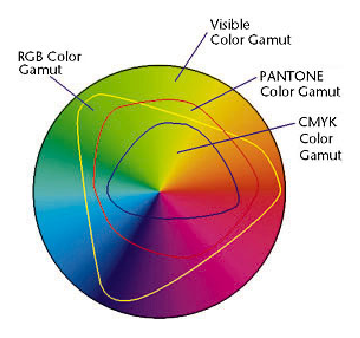
\includegraphics[width=0.4\textwidth]{gamuts}\qquad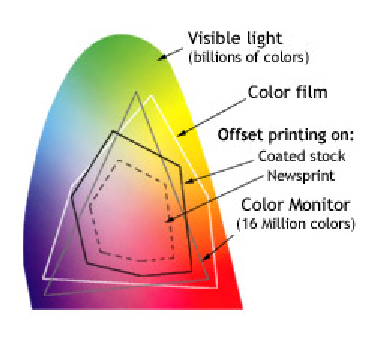
\includegraphics[width=0.4\textwidth]{spectrum}
\caption{\emph{Left:} A comparison of the colors available in various color
  spaces. \emph{Right:} A comparison of the colors available with various
  display technologies.}\label{fig:gamuts}
\end{figure}
%% websupport1.citytech.cuny.edu/faculty/phenry/gamuts.html. Currently 'Not found'.

%Dual product (print and electronic) or print-only journals:  CMYK format.
%Electronic-only journals:  RGB format.  
%Books: CMYK format.

\subsection{Requirements for graphics to be published in color}

\textbf{Graphics intended to be printed in color should be submitted in
 CMYK format. If you submit RGB files they will be converted to CMYK\@.}
 The AMS cannot guarantee that color reproduction in the print product will
 match the RGB file.

\ifjournal
 For electronic-only journals \emph{only}, RGB files are preferred.
\fi

\subsection{Color graphics to be printed in black and white or
 grayscale\texorpdfstring{\nopunct\ \ignorespaces}{}}
%	Color graphics to be printed in black and white or grayscale
 \textbf{should be converted to black and white or grayscale before
 being submitted to the AMS\@.}
 When color graphics are printed in black and white or grayscale, sometimes
 lighter colors, such as yellow, disappear, or darker colors, such as red
 and blue, appear to be the same tone. It is preferable that you convert
 your color graphics to grayscale and check to be sure that all the
 elements in your graphics print as desired---see
%        Figure~\ref{fig2gray}, page~\pageref{fig2gray}. Check your
 Figure~\ref{fig2gray}, \vpageref[above]{fig2gray}. Check your color
 figures on a black and white printer to ensure that the black and white
 printout of your figure is legible.

\begin{figure}[t]
\includegraphics{Color2Gray}
\caption{Colors don't always have the intended effect when converted to grayscale.}
\label{fig2gray}
\end{figure}

\subsection{Shades of colors} Inherently light colors should be handled
 carefully when using shades of them. Whereas 50\% red turns out to be a
 usable pink, a 50\% yellow or cyan may be almost invisible.

\subsection{Colored lines\texorpdfstring{\nopunct}{}} should be no less
 than .5 point in width. Colored lines in inherently light colors
 (e.g. yellow and cyan) should always be at or near 100\% in tint.

\needspace{4.5\baselineskip}

\secwnote[sec:tsize]{Using type in graphics}%
 {Type within graphics requires special attention to reproduce legibly.}

\begin{itemize}
\item Basic type size should be no less than 10 point at 100\%.
 Although 10-point type is acceptable for print, for graphics intended
 to be viewed online, screen resolution is 72 PPI and 10-point type
 will be difficult to read.
\item Do not put type on a dark background. 
 Dark type on dark colors is not legible.
\item Check your color figures on a black and white printer to ensure that
 the black and white printout of your figure is legible.
\end{itemize}

\secwnote[sec:tables]{Tables}%
{Tables can be thought of as a special kind of graphic. They often require
 a great deal of attention to make them effective.}

\begin{itemize}

\item Make sure that the width of the table does not exceed the width of
 the text block.

\item Very wide tables can be rotated using the \pkg{rotating} package
 together with the \env{sidewaystable} environment. Remember that tables
 (and figures) should be rotated such that the left-hand side of the table
 (or figure), after rotation, is at the bottom of the page.

\item Set table captions above the table.

\item For more help on the formatting of tables, see \cite[chapter 5]{MG}
 and \cite{voss-tbl}.
\end{itemize}

\secwnote[sec:photo]{Photographs}%
{Photographs must be at a minimum resolution of 300 dpi at the actual size
 that the photograph will be printed in the published product.}

\begin{itemize}
\item Photographs should be at least 300 dpi in resolution at the actual
 size that the photograph will be printed in the published product.  Do
 not scale photographs in \TeX.
\item File format can be EPS, TIFF, or JPEG.
\item Color photographs must be saved in CMYK format. (See Color graphics,
 section~\ref{sec:color}.)
\end{itemize}

\section{\TeX\ graphics}

There are several ways of providing graphics by the use of \TeX\ coding,
the principal choices being

\begin{description}
\item[tikz]Based on the PGF (portable graphics format), this is a very
 flexible environment for creating graphics within a \TeX\ document. Note
 that it functions equally well in dvips-based \latex/ and \pdfLaTeX/ as
 well as the newer varieties of \TeX\ such as \XeLaTeX/ and \LuaLaTeX/.
 The native documentation \cite{tkz} is excellent, though massive. There
 are two very good primers by Mertz and Slough: \cite{MeSlp} and
 \cite{MeSlt}. A large set of examples, often generously documented, can be
 found at \cite{tkz-ex}.
\item[pstricks]Also a very flexible and useful environment for drawing in
 \TeX. It is most easily used with dvips-based \TeX, though, with some
 care, it can be used with \pdfLaTeX/. There is an excellent reference
 book by Herbert Voss, \emph{PSTricks: Graphics and PostScript for \TeX\
 and \latex/} \cite{voss-pst}. The use of pstricks is also covered in some
 detail in \cite[chapters five and six]{GM}.
\item[xy and xypic]Though generally associated with commutative diagrams,
 these packages can also serve as a general drawing environment for \TeX.
\end{description}
\noindent A great deal of general information about other \latex/ graphics
packages can be found in \cite{GM}.

\section{Using a package to apply labels to graphics}

Several packages exist whose purpose is to place labels on graphics.
Use of such a package does ensure consistent fonts.  However, labels
added by such a package do not modify the dimensions of a graphic,
whether it is an EPS file or a drawing prepared by other means.

If labels are applied outside the edges of the graphic, they can
extend into the margin on the sides, or above or below the graphic
into space intended to separate the page content from the running head,
or the graphic from a caption.  In extreme cases, they can overprint
surrounding material, with no warning being issued.  Authors using
such packages should be alert to this possibility, and carefully check
the graphics where such labeling has been used.

If it is not possible to position labels within the boundaries of a
graphic, extra space should be added with \cn{vspace} to compensate.

\endinput


%%
%% This is file `Submitting2AMS.tex'
%% 
%% Copyright 2017 American Mathematical Society.
%% 
%% This file is part of the collection comprising the AMS Author Handbooks.
%% For details and license information, see the file README-AH.txt.
%%
%% The Current Maintainer of this work is the American Mathematical
%% Society.
%% 
%% ========================================================================
%% 

\chapter{Submitting files to the AMS}\label{ch:submit}

\section{Submission guidelines}

\noindent Upon acceptance of your 
\jmpm{article}{book}{paper}{\Memo}, the source file(s) should be sent
to the AMS office (this includes the \tex/ 
source file(s) and any graphics files).  Send
\emph{only} the files that are needed to process your submission or archive
it for future reference.  (This does \emph{not} include \fn{.log} or
\fn{.aux} files, for example.)

Before sending the source file(s), be sure you have proofread your 
\jmpm{article}{monograph}{paper}{\Memo\ submission} carefully. 
The files that you send must be the EXACT files
used to generate the proof copy that was accepted for publication.  In
order to avoid any possible production problems, before sending the files,
be sure to verify all items in the sections \textit{\nameref{sec:check}} (page~\pageref{sec:check}) and \textit{\nameref{sec:scheck}} (page~\pageref{sec:scheck}).

If your submission consists of \textbf{multiple files}, we recommend that
you bundle them using the Zip utility; this can be obtained (free) for
most platforms from \href{http://freecode.com}{\texttt{freecode.com}}\,.
Bundling means that only one (compressed) file needs to be sent, lessening
the chance of name conflicts or file corruption.

\section{Web server submissions (preferred)}
\noindent Accepted electronic manuscripts can be submitted via the web server
at\\
\href{http://www.ams.org/submit-book-journal}{\texttt{www.ams.org/submit-book-journal}}.
For security and confidentiality
reasons, submitting through the web server requires an AMS web account.
Authors who do not already have an account will be given the opportunity
to create one as they go through the submission process.

\section{Electronic mail submissions}
\noindent
Files sent by electronic mail should be addressed to
\texttt{pub-submit@ams.org}.  Include them as attachments, not as
part of the message.

The subject line of the message should use the publication code to identify the
\jmpm{journal (see the list of \textit{\nameref{tbl:series}}, page~\pageref{tbl:series}).}
{monograph series (see the list of \textit{\nameref{tbl:series}},
 page~\pageref{tbl:series}), and should include the name(s) of the author(s).}
{proceedings/collection series (see the list of \textit{\nameref{tbl:series}},
 page~\pageref{tbl:series}), and should include the name(s) of the editor(s).}
{as a \Memos\ submission.}
By including this information in the subject line, you will help speed up
the processing of your submission.

Submissions received through email will be acknowledged upon receipt by an
automatic reply while your submission is reviewed.  If there are any problems
with the file received, you will be notified.

\section{Other possibilities}
\noindent If your attempt to submit both through the web server and by
electronic mail fails, arrangements can be made for you to post your
files via FTP or on physical media.  Requests for help can be addressed
as described in the section ``\nameref{sec:amsresources}'' on
page~\pageref{sec:amsresources}.

\endinput


%%
%% This is file `ResourcesHelp.tex'
%% 
%% Copyright 2017 American Mathematical Society.
%% 
%% This file is part of the collection comprising the AMS Author Handbooks.
%% For details and license information, see the file README-AH.txt.
%%
%% The Current Maintainer of this work is the American Mathematical
%% Society.
%% 
%% ========================================================================
%% 

\chapter{Resources and getting help}\label{ch:resandhelp}

\enlargethispage{.5pc}

\phantomsection
\section{Getting help: AMS resources}\label{sec:amsresources}
\label{ch:amsresources}

Many questions raised by authors are answered in the AMS Author FAQ
\cite{FAQ}.  Please check there before asking for assistance.

\hypertarget{adr-tech-support}{}%
If you encounter difficulties in preparing or submitting your
manuscript in electronic form after it has been accepted for
publication by the appropriate editorial board, you can ask for help
from AMS Technical Support:

\medskip
\begingroup
\obeylines
Publications Technical Group
Phone: 800-321-4267, ext.\ 4080 \quad or \quad 401-455-4080
Email: \href{mailto:tech-support@ams.org}{\texttt{tech-support@ams.org}}
\endgroup
\medskip


All written correspondence should be sent to the appropriate AMS
department at:

\medskip
\begingroup
\obeylines
American Mathematical Society
201 Charles Street
Providence, RI \ 02904-2294 \ USA
\endgroup
\medskip

\noindent or by FAX to 401-331-3842.


%% instructions for journals or Memoirs
\ifmonograph
\else \ifproceedings
\else
\medskip
See submission instructions on the web starting from

\begingroup
\obeylines
\href{http://www.ams.org/authors/journal-list}{\texttt{www.ams.org/authors/journal-list}}
\endgroup
\fi\fi
%% end instructions for journals or Memoirs

%% instructions for books: monographs or proceedings/collections
\ifjournal
\else \ifmemoirs
\else
\medskip
\hypertarget{adr-acquisitions}{}Questions concerning what you need
to prepare your manuscript should be directed to:

\beginexample{\rm}
Acquisitions Department
Phone: 800-321-4267, ext.\ 4051\quad or\quad 401-455-4051
Email: \href{mailto:acquisitions@ams.org}{\texttt{acquisitions@ams.org}}
\endexample
\fi\fi
%% end instructions for books: monographs or proceedings/collections

\medskip
Problems in accessing the web server should be reported to:

\beginexample{\rm}
Email: \href{mailto:webmaster@ams.org}{\texttt{webmaster@ams.org}}
\endexample


\phantomsection
\section{\texorpdfstring{\protect\tex/}{TeX} resources}
\label{ch:texresources}

\latex/ and \tex/ are available on the web free of charge.
There are also several commercial \tex/ implementations.
AMS web pages devoted to \tex/ information can be accessed at
\href{http://www.ams.org/tex}{\texttt{www.ams.org/tex}}\,.
The first of these pages has links to other
pages that identify the various sources for the \tex/ program.

\latex/ is the most popular of the free front ends designed for use
with \tex/, the basic typesetting program.  Whereas plain \tex/
defines basic macros, \latex/ defines stylistic packages, setting up
styles for a monograph, journal article, and article in a proceedings
collection, which you can then alter to your own specifications.

\amslatex/ is a collection of \latex/ extensions that make various
kinds of mathematical constructions easier to produce and take more
care with certain finer details in order to yield publication-quality
results.  It consists of two parts: \pkg{amsmath} (the part concerned
with the mathematics) and \pkg{amscls}.
The latter is a collection of companion design
setup packages (variously referred to as `document class' or `class' files)
 that enable authors writing a monograph or article to
get largely the same visual appearance in their preliminary drafts as
in a final publication with the AMS\@.  Both parts of \amslatex/ are
included in the canonical \latex/ distribution as part of \TeX\,Live.

Updates for \pkg{amsmath} are best obtained from
\href{http://www.ctan.org/search.html}{CTAN};
updates for \pkg{amscls} can be obtained either from CTAN or from the
AMS web server at
\href{http://www.ams.org/tex}{\texttt{www.ams.org/tex}}\,.
Other AMS packages and collections are the AMSFonts and \pkg{amsrefs}.
These too are included in \TeX\,Live as well as available from both
the AMS web server and CTAN\@.  All distributions include a copy of
the relevant User's Guide and other related documentation in PDF form,
which can either be printed or viewed electronically.  (This
Author Handbook is the User's Guide to the \pkg{amscls} collection.)

The book \textit{More Math into \latex/} \cite{Gr} is written from the point
of view of a mathematician using \amslatex/, and contains many examples.
The \textit{Guide to \latex/}, fourth edition \cite{KD}, is a good
general introduction to \latex/.  The original and authoritative manual
 for \latex/ is the \textit{\latex/ User's Guide \& Reference Manual}
\cite{La}.  George Gr\"atzer has also written a series of articles for
\emph{Notices of the AMS} \cite{Gr1,Gr2,Gr3,Gr4,Gr5,Gr6,Gr7} that keeps
the interested user up-to-date with the latest developments in \latex/.

Another source of information on \tex/ and \latex/ is the \tex/ Users
Group (TUG)\@.  They can be contacted at:

\beginexample{\rm}
  \href{http://tug.org}{\tex/ Users Group}
  P.\,O.\,Box 2311
  Portland, OR 97208-2311
  (503) 223-9994, FAX: (206) 203-3960
  \href{mailto:office@tug.org}{\texttt{office@tug.org}}
\endexample

\noindent
TUG also distributes the \tex/ Live collection, which includes ready-to-run
implementations of \tex/ for Windows, Mac, and Unix platforms, as well as \latex/
%, \amstex/, 
and an extensive selection of packages, all freeware.

\section{Online assistance}

One of the best places to ask for assistance is the group known by the
acronym CTT,
\href{https://groups.google.com/forum/#!forum/comp.text.tex}{\texttt{groups.google.com/forum/comp.text.tex}}\,.
Most of the people who use CTT are more than willing to answer questions and give advice.

Another online source of assistance is
\href{http://tex.stackexchange.com}{\texttt{tex.stackexchange.com}}\,.
This is organized differently from most discussion groups. After signing
up, you pose and answer questions. In the process, you gain points
which in turn allow you to do more in the group. Be sure to read
\href{http://tex.stackexchange.com/about}{\texttt{tex.stackexchange.com/about}}
to get you started.

The AMS is not equipped to handle questions about specific platforms.
Links to sites providing such support, as well as addresses for discussion
lists and links for on-line forums, are given on this AMS web page:\\
\href{http://www.ams.org/tex/additional-sources}{\texttt{www.ams.org/tex/additional-sources}}.

\endinput


\backmatter

%%
%% This is file `AH_Bibliography.tex'
%% 
%% Copyright 2017 American Mathematical Society.
%% 
%% This file is part of the collection comprising the AMS Author Handbooks.
%% For details and license information, see the file README-AH.txt.
%%
%% The Current Maintainer of this work is the American Mathematical
%% Society.
%% 
%% ========================================================================
%% 

\renewcommand{\bibintro}{%
  Discounts are available on some of these books when they are ordered
  using information available on the \TeX\ Users Group page
  \href{https://www.tug.org/books/}{Books about TeX and Friends}.
  In particular, books published by Pearson affiliates (including
  Addison-Wesley) are eligible for a discount.}
  

\begin{thebibliography}{[ASMR]}

%\enlargethispage{2\baselineskip}
%\vspace*{-.75\baselineskip}
\raggedright

%\begin{extrabibtext}
%All documentation for AMS \tex/-related products is available in PDF
%form from the AMS web server as indicated below.  If you are reading
%this handbook on-line, the links for each item should be ``live''.
%\end{extrabibtext}

\bibitem[ABMR]{ABMR}
\href{http://www.ams.org/msnhtml/serials.pdf}
{\textit{Abbreviations of names of serials \textup[reviewed
in Mathematical Reviews\textup]}}, Amer. Math. Soc., Providence, RI.
\href{http://www.ams.org/msnhtml/serials.pdf}{\texttt{www.ams.org/msnhtml/serials.pdf}}

%\bibitem[AF]{AF} AMS Author FAQ,
%\url{www.ams.org/authors/author-faq}

\bibitem[AFG]{AFG} \href{ftp://ftp.ams.org/pub/tex/doc/amsfonts/amsfndoc.pdf}
{\textit{User's Guide to AMSFonts}}, version~2.2d,
Amer. Math. Soc.,  Providence, RI, 2002.  Link at
\href{http://www.ams.org/tex/amsfonts}{\texttt{www.ams.org/tex/amsfonts}}

\bibitem[AH]{AH} \textit{AMS Author Handbook},
Amer. Math. Soc., Providence, RI, 2014.  Link at
\href{http://www.ams.org/author-handbook}{\texttt{www.ams.org/author-handbook}}

\bibitem[AMG]{AMG} \href{http://mirrors.ctan.org/macros/latex/required/amsmath/amsldoc.pdf}{\textit{User's guide for the \pkg{amsmath} package
version~\textup{2.0}}}, Amer. Math. Soc., Providence, RI, and the \latex/3 Project, 2016.
\href{http://mirrors.ctan.org/macros/latex/required/amsmath/amsldoc.pdf}{\url{mirrors.ctan.org/macros/latex/required/amsmath/amsldoc.pdf}}
%\href{http://www.ams.org/tex/amslatex.html}{\texttt{www.ams.org/tex/amslatex}}

\bibitem[AMSR]{AMSR} \href{ftp://ftp.ams.org/pub/tex/amsrefs/amsrdoc.pdf}{\textit{User's Guide to the \pkg{amsrefs} Package}},
David Jones, Amer. Math. Soc., Providence, RI, 2013. Link at 
\href{http://www.ams.org/authors/amsrefs}{\texttt{www.ams.org/authors/amsrefs}}

%\bibitem[ATG]{ATG}
%\href{ftp://ftp.ams.org/pub/tex/doc/amstex/amsguide.pdf}
%{\textit{User's Guide to \amstex/}}, version~2.2,
%Amer. Math. Soc., Providence, RI, 2001.
%Link at \url{www.ams.org/tex/amstex}

\bibitem[ATH]{ATH}
\href{ftp://ftp.ams.org/pub/tex/doc/amscls/amsthdoc.pdf}
{\textit{Using the \texttt{amsthm} Package}},
version~2.20.2, Amer. Math. Soc., Providence, RI, 2015.  Link at 
\href{http://www.ams.org/tex/amslatex.html}{\texttt{www.ams.org/tex/amslatex}}

%\bibitem[ATP]{ATP} \textit{Using the \pkg{amsthm} package,
%version~\textup{2.0}}, Amer. Math. Soc., Providence, RI, 2004.\\
%Link at \url{www.ams.org/tex/amslatex.html}

\ifproceedings
\bibitem[EDP]{EDP}
\href{http://www.ams.org/publications/editpkg}
{Guide to AMS Editor's Package},
\url{www.ams.org/publications/editpkg}.
\fi

\bibitem[FAQ]{FAQ}
\href{http://www.ams.org/authors/author-faq}
{\textit{Frequently Asked Questions for AMS Authors}},
\url{www.ams.org/authors/author-faq}.
%%\url{www.ams.org/author-faq}.

%\bibitem[INT]{INT}
%\href{ftp://ftp.ams.org/pub/tex/doc/amstex/instr-t.pdf}
%{\textit{Instructions for Preparation of Papers and
%Monographs\textup{:} \amstex/}}, version~2.2b,
%Amer. Math. Soc., Providence, RI, 2002.
%Link at \url{www.ams.org/tex/amstex}

%\begin{extrabibtext}
%An extensive, up-to-date list of \tex/-related publications (both in print
%and electronic) appears on the web page
%\url{www.ams.org/tex/tex-pub} with links to sources where
%these publications can be obtained.
%\end{extrabibtext}

\bibitem[GM]{GM}  Michel Goossens, Frank Mittelbach et al.,
\textit{The \latex/ Graphics companion}, second ed., Addison-Wesley, Reading,
MA, 2007.

\bibitem[GGr]{GGr} George Gr\"atzer, \textit{Math into \latex/}, third ed.,
Springer, New York, 2000.

%\bibitem[Gr]{Gr} George Gr\"atzer, \textit{More Math into \latex/}, fourth ed.,
%Springer, New York, 2007.  (Supersedes \cite{GGr}.)

\bibitem[Gr]{Gr} George Gr\"atzer, \textit{More Math into \latex/}, fifth ed.,
Springer, New York, 2016.  (Supersedes \cite{GGr}.)

\bibitem[Gr1]{Gr1}
G.~Gr{\"a}tzer.
\newblock What is new in \latex/? I. Breaking free.
\newblock {\em Notices of the AMS}, 56(1):52--54, January 2009.
\href{http://www.ams.org/notices/200901/tx090100052p.pdf}{\texttt{www.ams.org/notices/200901/tx090100052p.pdf}}

\bibitem[Gr2]{Gr2}
G.~Gr{\"a}tzer.
\newblock What is new in \latex/? II. \tex/ implementations, evolution or
  revolution.
\newblock {\em Notices of the AMS}, 56(5):627--629, May 2009.
\href{http://www.ams.org/notices/200905/rtx090500627p.pdf}{\texttt{www.ams.org/notices/200905/rtx090500627p.pdf}}

\bibitem[Gr3]{Gr3}
G.~Gr{\"a}tzer.
\newblock What is new in \latex/? III. Formatting references.
\newblock {\em Notices of the AMS}, 56(8):954--956, September 2009.
\href{http://www.ams.org/notices/200908/rtx090800954p.pdf}{\texttt{www.ams.org/notices/200908/rtx090800954p.pdf}}

\bibitem[Gr4]{Gr4}
G.~Gr{\"a}tzer.
\newblock What is new in \latex/? IV. WYSIWYG \latex/.
\newblock {\em Notices of the AMS}, 58(6):828--830, June/July 2011.
\href{http://www.ams.org/notices/201106/rtx110600828p.pdf}{\texttt{www.ams.org/notices/201106/rtx110600828p.pdf}}

\bibitem[Gr5]{Gr5}
G.~Gr{\"a}tzer.
\newblock What is new in \latex/? V. \latex/ on an iPad. Foundation.
\newblock {\em Notices of the AMS}, 60(3):332--334, March 2013.
\href{http://www.ams.org/notices/201303/rnoti-p332.pdf}{\texttt{www.ams.org/notices/201303/rnoti-p332.pdf}}

\bibitem[Gr6]{Gr6}
G.~Gr{\"a}tzer.
\newblock What is new in \latex/? VI. \latex/ on an iPad. Empire.
\newblock {\em Notices of the AMS}, 60(4):434--439, April 2013.
\href{http://www.ams.org/notices/201304/rnoti-p434.pdf}{\texttt{www.ams.org/notices/201304/rnoti-p434.pdf}}

\bibitem[Gr7]{Gr7}
G.~Gr{\"a}tzer.
\newblock What is new in \latex/? VII. The STIX math symbols.
\newblock {\em Notices of the AMS}, 62(6):667--669, June/July 2015.
\href{http://www.ams.org/notices/201506/rnoti-p667.pdf}{\texttt{www.ams.org/notices/201506/rnoti-p667.pdf}}

\bibitem[Hi]{Hi} Nicholas J. Higham, \textit{Handbook of Writing for
the Mathematical Sciences}, second ed., SIAM, Philadelphia, PA, 1998.

\bibitem[KD]{KD} Helmut Kopka and Patrick W. Daly, \textit{Guide to \latex/},
fourth ed., Addison-Wesley, Boston, 2004.

\bibitem[Kn]{Kn} Donald E. Knuth, \textit{The \TeX book},
Addison-Wesley, Reading, MA, 1984.

\bibitem[La]{La} Leslie Lamport, \textit{\LaTeX{\textup:} A document
preparation system}, second ed., Addison-Wesley, Reading, MA, 1994.

\bibitem[LW]{LW} Mary Letourneau and Jennifer Wright Sharp,
\textit{AMS style guide: Journals}, Amer. Math. Soc., Providence, RI, 2017.
\href{http://www.ams.org/publications/authors/AMS-StyleGuide-print.pdf}{\texttt{www.ams.org/publications/authors/AMS-StyleGuide-print.pdf}}

\bibitem[MeSlp]{MeSlp}
Andrew Mertz, William Slough,
\emph{Graphics with \TikZ},
Prac\tex/ Journal, \textbf{2007}:1.
\href{http://tug.org/pracjourn/2007-1/mertz/mertz.pdf}{\texttt{tug.org/pracjourn/2007-1/mertz/mertz.pdf}}

\bibitem[MeSlt]{MeSlt}
Andrew Mertz, William Slough,
\emph{Graphics with \textsc{pgf} and \TikZ},
TUGboat, \textbf{28}:1 (2007), 91--99.
\href{http://tug.org/TUGboat/tb28-1/tb88mertz.pdf}{\texttt{tug.org/TUGboat/tb28-1/tb88mertz.pdf}}

\bibitem[MG]{MG} Frank Mittelbach, Michel Goossens, et al.,
\textit{The \latex/ companion}, second ed., Addison-Wesley, Reading,
MA, 2004.  This is now also available as an ebook, in both English and
German; see the TUG web page cited above.  The front matter, including
the full Table of Contents, can be viewed online, at
\href{https://www.latex-project.org/help/books/tlc2-ch0.pdf}{\texttt{www.latex-project.org/help/books/tlc2-ch0.pdf}}.

\bibitem[MSC]{MSC}
2010 Mathematics Subject Classification
\href{http://www.ams.org/msc}{\texttt{www.ams.org/msc}}.

\bibitem[SHSD]{SHSD}
Norman E. Steenrod, Paul R. Halmos, Menahem M. Schiffer, and Jean A.
Dieudonn\'e, \textit{How to write mathematics}, 6th printing (2000),
Amer. Math. Soc., Providence, RI, 1973, reprinted with corrections 1981.

\bibitem[Sw]{Sw} Ellen E. Swanson, 
%\href{ftp://ftp.ams.org/pub/author-info/documentation/howto/mit-2.pdf}
\href{http://www.ams.org/publications/authors/mit-2.pdf}
{\textit{Mathematics into type}},
updated ed., Amer. Math. Soc., Providence, RI, 1999.  Link at
\href{http://www.ams.org/publications/authors}{\texttt{www.ams.org/authors}}

\bibitem[tkz]{tkz}
Till Tantau,
The \TikZ\ and PGF Packages: Manual for version 3.0.1a, 
2013.
\href{http://www.ctan.org/tex-archive/graphics/pgf/base/doc/pgfmanual.pdf}{\texttt{www.ctan.org/tex-archive/graphics/pgf/base/doc/pgfmanual.pdf}}

\bibitem[tkz-ex]{tkz-ex}
Online gallery of \TikZ\ and PGF examples.
\href{http://www.texample.net/tikz/examples/all/}{\texttt{www.texample.net/tikz/examples/all/}}

\bibitem[voss-pst]{voss-pst}
Herbert Voss,
PSTricks: Graphics and PostScript for \TeX\ and \LaTeX,
UIT Cambridge Ltd.,
2011.

\bibitem[voss-tbl]{voss-tbl}
Herbert Voss,
Typesetting Tables with \LaTeX,
UIT Cambridge Ltd.,
2010.

\end{thebibliography}

\endinput


\end{document}
